% !TEX program = xelatex
%%%%%%%%%%%%%%%%%%%%%%%%

\documentclass[11pt,aspectratio=169]{beamer} % 11pt is default
\usetheme{metropolis} % [progressbar=frametitle]
\setbeamercolor{background canvas}{bg=white}
\setbeamertemplate{caption}{\insertcaption} 
\setbeamersize{text margin left=2em,text margin right=2em}
\setbeamertemplate{frame footer}{\vspace{-5pt}}

\usepackage[round]{natbib}
\usepackage{amsmath}
\usepackage{mathtools}
\usepackage[group-minimum-digits=4,group-separator={,}]{siunitx}
\usepackage{graphicx}
\usepackage{wrapfig}
\usepackage{multimedia}

\usepackage{tikz}
\usetikzlibrary{backgrounds}
\usetikzlibrary{arrows,shapes}
\usetikzlibrary{tikzmark}
\usetikzlibrary{calc}
\usepackage[dvipsnames]{xcolor}

\usepackage[skins,theorems]{tcolorbox}
\usepackage{pdfpages}
\usepackage{colortbl}
\usepackage{changepage}
\usepackage{booktabs}
\usepackage{makecell}
\usepackage{setspace}
\usepackage{algorithm}
\usepackage[noend]{algpseudocode}
\usepackage{subcaption}
\usepackage[framemethod=TikZ]{mdframed}
\usepackage{xspace}

\usepackage{annotate-equations}

% Shortcut for beamer frames
\newcommand{\bframe}[2][c]{\begin{frame}[#1]{#2}}
\newcommand{\eframe}{\end{frame}} % \eframe causes problems for some reason

% Shortcut for bold text
\newcommand{\fat}[1]{\textbf{#1}}

% Boxing items on slide
\newcommand{\Cboxed}[2]{\colorlet{currentcolor}{.}{\color{#1}\fbox{\color{currentcolor}#2}}} %create coloured box around equation

% checkmark and xmark
\usepackage{pifont}
\newcommand{\cmark}{\ding{51}}%
\newcommand{\xmark}{\ding{55}}%

% Highlighting text in orange
\newcommand{\e}[1]{\alert{#1}}

% Underline
\newcommand{\uline}[1]{\underline{#1}}

% Include figure
\newcommand{\imgw}[2]{\includegraphics[width=#2\textwidth]{#1}} % \imgw{file}{height-scale}
\newcommand{\imgh}[2]{\includegraphics[height=#2\textheight]{#1}} % \imgh{file}{width-scale}

% Shortcut for latex commands
\newcommand{\blist}{\vspace{-3pt}\begin{list}{\raisebox{1pt}{\small$\bullet$}}{\leftmargin=13pt\itemsep=4pt}}
\newcommand{\blisttab}{\vspace{5pt}\blist}
\newcommand{\elisttab}{\end{list}}
\newcommand{\listtab}{\\[3pt] $\Rightarrow$ }
\newcommand{\elist}{\end{list}\vspace{5pt}}
\newcommand{\bblock}[1]{\metroset{block=fill}\begin{block}{#1}}
\newcommand{\eblock}{\end{block}}
\newcommand{\bmath}[1][0]{\begin{equation*}\hspace{#1em}}
\newcommand{\emath}{\end{equation*}}
\newcommand{\bcol}{\begin{columns}}
\newcommand{\col}[1]{\column{#1\textwidth}}
\newcommand{\tcol}[1]{\column[T]{#1\textwidth}}
\newcommand{\ecol}{\end{columns}}
\newcommand{\place}[4]{\begin{textblock}{#3}(#1,#2) #4 \end{textblock}} % \place{x}{y}{width}{text}
\newcommand{\placeframed}[4]{\place{#1}{#2}{#3}{\fbox{\parbox{#3em}{#4}}}}
\newcommand{\placeimg}[4]{\place{#1}{#2}{#3}{\imgw{#4}{1}}} % \placeimg{x}{y}{width}{file}
\newcommand{\videolink}[2]{\movie[externalviewer]{{\bf Video:} #1}{videos/#2}} % \videolink{title}{file}
\newcommand{\btab}[1]{\begin{tabular}{#1}}
\newcommand{\etab}{\end{tabular}}
\newcommand{\balgo}[2][1.3]{{#2:} \\[5pt] \begin{algorithmic}[1] \linespread{#1}\selectfont}
\newcommand{\ealgo}{\end{algorithmic}}
\renewcommand{\algorithmicloop}{\textbf{repeat:}}
\newcommand{\cred}{\cellcolor{red!25}}
\newcommand{\cgreen}{\cellcolor{green!25}}

% Shortcut for commonly used math symbols
\newcommand{\condpr}[2]{\text{Pr}\hspace{-1pt}\left\{ #1 \ \mid \ #2 \right\}}
\newcommand{\exarg}[2]{\mathbb{E}_{#1}\hspace{-2pt}\left[ #2 \right]}
\newcommand{\exnoarg}[1]{\mathbb{E}_{#1}}
\NewDocumentCommand\ex{ m g }{
	\IfNoValueTF{#2}{\exnoarg{#1}}{\exarg{#1}{#2}}
}
\newcommand{\der}[2]{\frac{\partial #1}{\partial #2}}
\newcommand{\stats}{\mathcal{S}}
\newcommand{\acts}{\mathcal{A}}
\newcommand{\rews}{\mathcal{R}}
\newcommand{\eps}{\mathcal{E}}
\newcommand{\ver}{\,\vert\,}
\newcommand{\vhat}{\hat{v}}
\newcommand{\qhat}{\hat{q}}
% \newcommand{\para}{\textbf{w}}
\newcommand{\feats}{\textbf{x}}
\newcommand{\elig}{\textbf{z}}
\newcommand{\gradient}{\nabla}
\newcommand{\outline}{Lecture Outline}
\newcommand{\reading}{Reading}
\newcommand{\h}[1]{\emph{#1}}

\emph
% \newcommand{\lindex}[1]{%
% 	\lowercase{\def\temp{#1}%
% 	\expandafter\index\expandafter{\temp}%
% }

\newcommand{\indx}[1]{\index{#1}}
\newcommand{\hind}[1]{\h{#1}\lindex{#1}}

% Set of real numbers
\newcommand{\R}{\mathbb{R}}
% Proportional to
% Transpose of a vector x
\newcommand{\vectranspose}[1]{#1^\top}
% Transpose of a matrix X
\newcommand{\mattranspose}[1]{#1^\top}
% Probability
\newcommand{\pr}{\text{Pr}}
% Conditional probability of x given y
\newcommand{\cpr}[2]{\pr( #1 \mid #2 )}
% x sampled according to probability distribution p
\newcommand{\sampled}[2]{#1 \sim #2}
% Assign value y to variable x
\newcommand{\assign}[2]{#1 \gets #2}
% Training data set
\newcommand{\data}{\mathcal{D}}
% Concatenation of inputs a, b, c, ...
\newcommand{\con}[1]{\langle #1 \rangle}
% array with bracket
\newcommand{\bra}[2]{\left[ \begin{array}{#1} #2 \end{array} \right]}
% Indicator function: returns 1 if x is true, otherwise returns 0
\newcommand{\ind}[1]{[#1]_1}

% common way of referring to places
\newcommand{\seehere}[1]{(\cref{#1})}

% shortcut text commands
\newcommand{\rl}{RL\xspace}
\newcommand{\marl}{MARL\xspace}
\newcommand{\ctde}{CTDE\xspace}
\newcommand{\sa}{single-agent\xspace}
\newcommand{\ma}{multi-agent\xspace}
\newcommand{\Ma}{Multi-agent\xspace}
\newcommand{\mas}{multi-agent system\xspace}
\newcommand{\stat}{stationarity\xspace}
\newcommand{\nonstat}{non-stationarity\xspace}
\newcommand{\pg}{policy gradient\xspace}
\newcommand{\vb}{value-based\xspace}
\newcommand{\pbt}{population-based training\xspace}
\newcommand{\psro}{policy space response oracles\xspace}
\newcommand{\Psro}{Policy space response oracles\xspace}
\newcommand{\sct}{\emph{StarCraft~II}\xspace}
\newcommand{\as}{AlphaStar\xspace}
\newcommand{\az}{AlphaZero\xspace}
\newcommand{\lbf}{level-based foraging\xspace}
\newcommand{\Lbf}{Level-based foraging\xspace}
\newcommand{\nfg}{normal-form game\xspace}
\newcommand{\nfgs}{normal-form games\xspace}
\newcommand{\Nfg}{Normal-form game\xspace}
\newcommand{\Nfgs}{Normal-form games\xspace}
\newcommand{\rps}{Rock-Paper-Scissors\xspace}
\newcommand{\pd}{Prisoner's Dilemma\xspace}
\newcommand{\survey}[4]{\noindent #1 (#4). ``#2.'' In: {\it #3}. \\}
\newcommand{\nashprob}{\textsc{Nash}\xspace}
\newcommand{\eol}{\textsc{End-of-Line}\xspace}
\newcommand{\ul}[1]{\underline{#1}}
\newcommand\norm[1]{\lVert#1\rVert}
\newcommand{\qlearn}{Q-learning\xspace}
\newcommand{\sarsa}{Sarsa\xspace}
\newcommand{\bayes}{Bayesian\xspace}
\newcommand{\bellman}{Bellman\xspace}
\newcommand{\markov}{Markov\xspace}
\newcommand{\pareto}{Pareto\xspace}
\newcommand{\boltzmann}{Boltzmann\xspace}
\newcommand{\mc}{Monte Carlo\xspace}
\newcommand{\nash}{Nash\xspace}
\newcommand{\ppad}{PPAD}
\newcommand{\dqn}{deep Q-networks\xspace}
\newcommand{\reinforce}{REINFORCE\xspace}
\newcommand{\qmix}{QMIX\xspace}
\newcommand{\qtran}{QTRAN\xspace}
\newcommand{\adam}{Adam\xspace}
\newcommand{\nret}{{$N$}-step returns\xspace}

% COMMANDS FOR COMMON NOTATION

% agent set
% state space
\newcommand{\St}{S}
\newcommand{\Stterm}{\bar{\St}}
% state
\newcommand{\st}{s}
\newcommand{\sth}{\hat{\st}}
% observation space
\newcommand{\Ob}{O}

% observation
\newcommand{\ob}{o}

% joint observation
\newcommand{\job}{o}
% action space
\newcommand{\Ac}{A}

% action
\newcommand{\ac}{a}
\newcommand{\ach}{\hat{\ac}}

% joint action
\newcommand{\jac}{a}
% reward
\newcommand{\rew}{r}
\newcommand{\rewh}{\hat{\rew}}
% centralised information
\newcommand{\ci}{z}

% initial state distribution

\newcommand{\instdist}{\mu}
% % state transition function

\newcommand{\Stf}{\mathcal{T}}
% % simulation/sampling model
\newcommand{\Stfsim}{\widehat{\Stf}}

% observation function
\newcommand{\Obf}{\mathcal{O}}

% reward function
\newcommand{\Rew}{\mathcal{R}}

% POLICIES, RETURNS, VALUES

% policy space
\newcommand{\Pol}{\Pi}

% policy
\newcommand{\pol}{\pi}
\newcommand{\poltil}{\tilde{\pol}}

% set of histories
\newcommand{\His}{H}
\newcommand{\Fhis}{\hat{\His}}
% history
\newcommand{\his}{h}

% full history
\newcommand{\fhis}{\hat{\his}}

% observation history extracted from full history
\newcommand{\obsext}{\sigma}

% discount factor
\newcommand{\dsc}{\gamma}

% return
\newcommand{\ret}{u}

% expected return for joint policy
\newcommand{\exret}{U}

% Agents
\newcommand{\Ag}{I}

% RL / MARL

% learning algorithm

\newcommand{\alg}{\mathbb{L}}

% empirical distribution/ average policy
\newcommand{\empdis}{\bar{\pol}}
\newcommand{\avgpol}{\bar{\pol}}
\newcommand{\agmod}{\hat{\pol}}
\newcommand{\Agmod}{\hat{\Pol}}
\newcommand{\agmodj}{agent model for agent $j$}

% best response
\newcommand{\br}{\textnormal{BR}}

% game value
\newcommand{\gval}{Value}

% value under agent model
\newcommand{\amval}{AV}

% regret
\newcommand{\regret}{Regret}
\newcommand{\avgreg}{\bar{R}}
% TD target
\newcommand{\target}{\mathcal{X}}
% step size (for gradient-based MARL in Chapter 5)
\newcommand{\step}{\kappa}


% DEEP LEARNING

% parameters
\newcommand{\para}{\theta}

% loss
\newcommand{\loss}{\mathcal{L}}
% batch
\newcommand{\batch}{\mathcal{B}}
\newcommand{\batchsize}{B}

% etnropy
\newcommand{\entropy}{\mathcal{H}}

% Create algorithm environment
\newcommand{\balg}[2]{
  \begin{algorithm}[H]
    \caption{#1}
    \label{alg:#2}
    \setstretch{1.1}
    \begin{algorithmic}[1]}

\newcommand{\ealg}{
    \end{algorithmic}
  \end{algorithm}}

% Argmin/ Argmax operators

\DeclareMathOperator*{\argmin}{arg\,min} 
\DeclareMathOperator*{\argmax}{arg\,max}

\makeatletter
\newenvironment{myitemize}{%
   \setlength{\topsep}{0pt}
   \setlength{\partopsep}{0pt}
   \renewcommand*{\@listi}{\leftmargin\leftmargini \parsep\z@ \topsep\z@ \itemsep\z@}
   \let\@listI\@listi
   \itemize
}{\enditemize}
\makeatother  

% define widebar for target parameters
\makeatletter
\newcommand*\rel@kern[1]{\kern#1\dimexpr\macc@kerna}
\newcommand*\widebar[1]{%
	\begingroup
	\def\mathaccent##1##2{%
		\rel@kern{0.8}%
		\overline{\rel@kern{-0.8}\macc@nucleus\rel@kern{0.2}}%
		\rel@kern{-0.2}%
	}%
	\macc@depth\@ne
	\let\math@bgroup\@empty \let\math@egroup\macc@set@skewchar
	\mathsurround\z@ \frozen@everymath{\mathgroup\macc@group\relax}%
	\macc@set@skewchar\relax
	\let\mathaccentV\macc@nested@a
	\macc@nested@a\relax111{#1}%
	\endgroup
}
\makeatother


% MATRIX GAMES

\newcolumntype{?}{!{\vrule width 1pt}}
\newcommand{\bhline}{\Xhline{1pt}}
\newcommand{\gametwo}[3]{
	\begin{tabular}{c?c|c}
		 & #1 \\
		\bhline
		#2    \\
		\hline
		#3    \\
	\end{tabular}
}
\newcommand{\gamethree}[4]{
	\begin{tabular}{c?c|c|c}
		 & #1 \\
		\bhline
		#2    \\
		\hline
		#3    \\
		\hline
		#4    \\
	\end{tabular}
}

\newcommand{\gamepd}{
    % \gametwo{C & D}{C & -1,-1 & -5,0}{D & 0,-5 & -3,-3}
	\begin{tabular}{c|c|c}
	& C & D \\
	\hline
	C & -1,-1 & -5,0 \\
	\hline
	D & 0,-5 & -3,-3
	\end{tabular}
}

\newcommand{\gamerps}{
    % \gamethree{R & P & S}{R & 0,0 & -1,1 & 1,-1}{P & 1,-1 & 0,0 & -1,1}{S & -1,1 & 1,-1 & 0,0}
	\begin{tabular}{c|c|c|c}
	& R & P & S \\
	\hline
	R & 0,0 & -1,1 & 1,-1 \\
	\hline
	P & 1,-1 & 0,0 & -1,1 \\
	\hline
	S & -1,1 & 1,-1 & 0,0
	\end{tabular}
}

\newcommand{\gamecoord}{
    % \gametwo{A & B}{A & 10 & 0}{B & 0 & 10}
	\begin{tabular}{c|c|c}
		& A & B \\
		\hline
		A & 10 & 0 \\
		\hline
		B & 0 & 10 \\
	\end{tabular}
}

\newcommand{\gamechicken}{
    % \gametwo{S & L}{S & 0,0 & 7,2}{L & 2,7 & 6,6}
	\begin{tabular}{c|c|c}
		& S & L \\
		\hline
		S & 0,0 & 7,2 \\
		\hline
		L & 2,7 & 6,6
	\end{tabular}
}

\newcommand{\gamestaghunt}{
    % \gametwo{S & H}{S & 4,4 & 0,3}{H & 3,0 & 2,2}
	\begin{tabular}{c|c|c}
		& S & H \\
		\hline
		S & 4,4 & 0,3 \\
		\hline
		H & 3,0 & 2,2
	\end{tabular}
}

\newcommand{\gamebattle}{
    \begin{tabular}{c|c|c}
    & A & B \\
    \hline
    A & 10,7 & 2,2 \\
    \hline
    B & 0,0 & 7,10
    \end{tabular}
}

\newcommand{\gameepsne}{
    % \gametwo{C & D}{A & 100,100 & 0,0}{B & 1,2 & 1,1}
	\begin{tabular}{c|c|c}
		& C & D \\
		\hline
		A & 100,100 & 0,0 \\
		\hline
		B & 1,2 & 1,1
	\end{tabular}
}

% Define colorboxes
\tcbset{
  % Defaults
  my box/main style/.style={},
  my box/title style/.style={},
  % Use the 'append' variants if you want to add to the defaults instead of
  % overriding them.
  my box/main/.style={/tcb/my box/main style/.style={#1}},
  my box/title/.style={/tcb/my box/title style/.style={#1}},
  my box/append main/.style={/tcb/my box/main style/.append style={#1}},
  my box/append title/.style={/tcb/my box/title style/.append style={#1}},
  %
  my box/.style={
    my box/.cd, #1,
    /tcb/.cd,
    enhanced,
    my box/main style,
    attach boxed title to top left={xshift=0.2cm, yshift=-0.2cm},
    top=10pt,
    boxed title style={
      outer arc=0pt,
      arc=0pt,
      top=3pt,
      bottom=3pt,
      my box/title style,
    },
  },
}

% define 'solutionbox' environment with coloured box
\newtcolorbox{solutionbox}[1][]{
  my box={
    main={colframe=green!40!gray!90, colback=green!20!gray!5},
    title={colback=green!40!gray!90},
  },
  title=Solution,
  #1,
}

\newtcolorbox{problembox}[1][]{
  my box={
    main={colframe=red!40!gray!90, colback=red!20!gray!5},
    title={colback=red!40!gray!90},
  },
  title=Problem,
  #1,
}

\newtcolorbox{notebox}[1][]{
  my box={
    main={colframe=orange!40!gray!80, colback=orange!20!gray!5},
    title={colback=orange!40!gray!80},
  },
  title=Note,
  #1,
}

\newtcolorbox{intuitionbox}[1][]{
  my box={
    main={colframe=blue!60!gray!80, colback=blue!20!gray!5},
    title={colback=blue!60!gray!80},
  },
  title=Intuition,
  #1,
}

\newtcolorbox{reminderbox}[1][]{
  my box={
    main={colframe=black!40!gray, colback=gray!10!white},
    title={colback=black!40!gray},
  },
  title=Reminder,
  #1,
}

\newtcolorbox{custombox}[2][]{
  my box={
    main={colframe=black!40!gray, colback=gray!10!white},
    title={colback=black!40!gray},
  },
  title={#2},
  #1,
}

% no title boxes
\newtcolorbox{greenbox}[1][]{
  my box={
    main={colframe=green!40!gray!90, colback=green!20!gray!5},
  },
  #1,
}
\newtcolorbox{redbox}[1][]{
  my box={
    main={colframe=red!40!gray!90, colback=red!20!gray!5},
  },
  #1,
}
\newtcolorbox{orangebox}[1][]{
  my box={
    main={colframe=orange!40!gray!80, colback=orange!20!gray!5},
  },
  #1,
}
\newtcolorbox{bluebox}[1][]{
  my box={
    main={colframe=blue!60!gray!80, colback=blue!20!gray!5},
  },
  #1,
}
\newtcolorbox{blackbox}[1][]{
  my box={
    main={colframe=black!55!black, colback=gray!5!white},
  },
  #1,
}


% Define intro slide command
\newcommand{\introslide}{
    \begin{frame}{MARL Book}
        \begin{columns}
            \begin{column}{0.5\textwidth}
            \begin{figure}
              \centering
              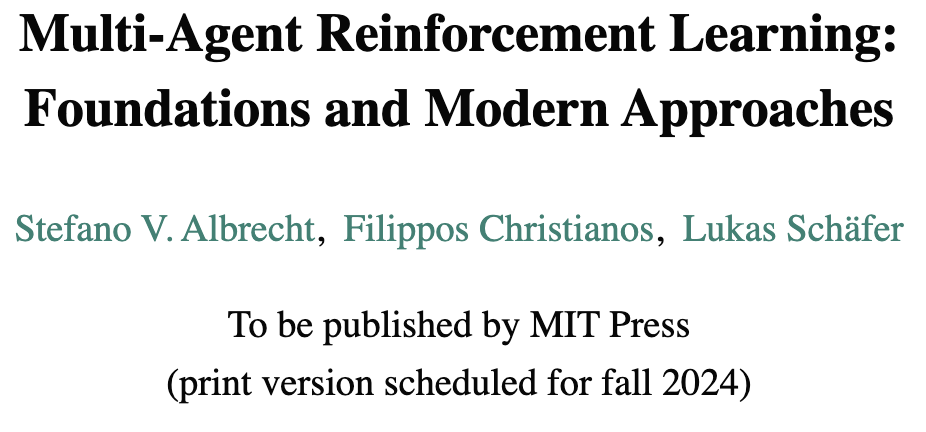
\includegraphics[width=\textwidth,height=.8\textheight,keepaspectratio]{images/1_MARL_book.png}
            
              \label{fig:enter-label}
            \end{figure}
          \end{column}
        
        \hspace{20pt}
            
          % Column for the text
            \begin{column}{0.45\textwidth}
	        \small

                This lecture is based on \textit{Multi-Agent Reinforcement Learning: Foundations and Modern Approaches} by Stefano V. Albrecht, Filippos Christianos and Lukas Sch\"afer
                
                \vspace{20pt}
                
                The book can be downloaded for free at \textcolor{blue}{\href{https://www.marl-book.com/}{www.marl-book.com}}.
            \end{column}
        
        \end{columns}
    \end{frame}
}

\newcommand{\leoslide}{
  \author{Stefano V. Albrecht, Filippos Christianos, Lukas Sch\"afer \\ Slides by: Leonard Hinckeldey}
}

\newcommand{\otherslide}{
  \author{Stefano V. Albrecht, Filippos Christianos, Lukas Sch\"afer}
}
	
\title{Multi-Agent Reinforcement Learning}
\date{}

\hypersetup{
  pdfsubject = {Multi-Agent Reinforcement Learning},
}

\leoslide

\subtitle{Solution Concepts for Games}

\begin{document}
\maketitle

\introslide

\begin{frame}{\outline}

\blist
    \item Joint policy and expected return
    \item Equilibrium solution concepts
    \item Additional solution criteria 
    \item Complexity of computing equilibria
\elist
    
\end{frame}

\begin{frame}{Solution Concepts for Games}
	\begin{center}
        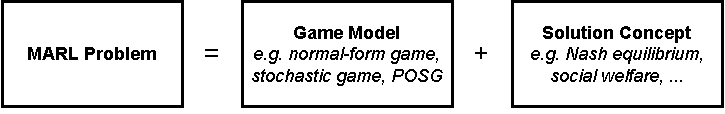
\includegraphics{images/chapter_4/marl-learning-problem.pdf}
   	\end{center}
    	
    What does it mean to act \e{optimally} in a multi-agent system?

    \blist
        \item Maximizing returns of one agent is no longer enough to determine a solution
        \item We must consider the {\bf joint policy} of all agents
        \item This is less straightforward, and there are many different solution concepts
    \elist
    
\end{frame}

\section{Joint Policy and Expected Return}

\begin{frame}{Joint Policy}

    The joint policy is the combination of all agents' policies. 

    \blist
        \item \(\pi = (\pi_1, ..., \pi_n)\) is the joint policy 
    \elist

    The probability of a joint action under joint policy $\pi$ can be defined as:

    \[
        \pi(a^{\tau}|h^{\tau}) = \prod_{j \in I}\pi_{j}(a_{j}^\tau | h^{\tau}_j)
    \]

    \begin{notebox}
        This definition assumes probabilistic independence between agents' policies. 
    \end{notebox}

\end{frame}

\begin{frame}{Additional Notation}

    In the multi-agent setting, we add the following notation: 

    \blist
        \item \(\hat{h} = \{(s^{\tau}, o^{\tau}, a^{\tau})_{\tau = 0}^{t-1}, s^t, o^t\}\) is the \fat{full history} containing:
        \blist
            \item \(s^\tau\), states up to \(t-1\)
            \item \(o^\tau\), joint observations up to \(t-1\)
            \item  \(a^{\tau}\), joint actions up to \(t-1\)
            \item \(s^t\) and \(o^t\) at current time step \(t\)
        \elist
        \item \(\sigma(\hat{h}^t) = (o^0, ..., o^t)\) is a function that returns the joint observation history from the \fat{full history} 
        \item \(\mathcal{O}(o^t|a^{t-1}, s^t)\) is the joint observation probability
    \elist
    
\end{frame}

\begin{frame}{History Based Expected Return}

    Given a joint policy \(\pi\), we can define the expected return for agent \(i\) under \(\pi\) as the probability-weighted sum of returns for agent \(i\) under all possible \fat{full histories.}
    \vspace{5pt}
    \blist
        \item Let $\hat{H}$ be a set containing all full histories $\hat{h}^t$ for $t \to \infty$
        \item then the expected return for agent $i$ under joint policy \(\pi\) is given by:
    \elist
    \vspace{0pt}
    \begin{align*}
         U_i(\pi) &= \lim_{t \to \infty} \mathbb{E}_{\hat{h}^t \sim (\mu, \mathcal{T}, \mathcal{O}, \pi)}\left[u_{i}(\hat{h}^t) \right] \\[5pt]
         &= \sum_{\hat{h}^t \in \hat{H}} \Pr(\hat{h}^t|\pi)u_i(\hat{h}^t)
    \end{align*}


        
\end{frame}

\begin{frame}{History Based Expected Return - Continued}

    The probability of a full history $\Pr(\hat{h}^t|\pi)$ is:
    \vspace{2pt}
    \[
        \Pr(\hat{h}^t | \pi) = \mu(s^0)\mathcal{O}(o^0 | \emptyset, s^0) \prod_{\tau=0}^{t-1} \pi(a^\tau | \hat{h}^\tau)\mathcal{T}(s^{\tau+1} | s^\tau, a^\tau)\mathcal{O}(o^{\tau+1} | a^\tau, s^{\tau+1})
    \]

    \(u_i(\hat{h}^t)\) is the discounted return for agent \(i\) in the \fat{full history}

    \[
        u_i(\hat{h}^t) = \sum_{\tau=0}^{t-1} \gamma^\tau R_i(s^\tau, a^\tau, s^{\tau+1})
    \]
    
\end{frame}

\begin{frame}{Recursive Expected Returns}

    Expected returns under a \fat{joint policy} can also be defined recursively, analogously to the Bellman recursion. 
        \vspace{2pt}
    \[
        V^{\pi}_i(\hat{h}) = \sum_{a \in A} \pi(a \mid \sigma(\hat{h})) Q^{\pi}_i (\hat{h}, a)
    \]

    We can use this to define a \(Q\) function for the individual agent \(i\) as follows:
    \vspace{2pt}
    \[
        Q^{\pi}_i(\hat{h}, a) = \sum_{s' \in S} \mathcal{T}(s' \mid s(\hat{h}), a) \left[ \mathcal{R}_i(s(\hat{h}), a, s') + \gamma \sum_{o' \in O} O(o' \mid a, s') V^{\pi}_i(\langle \hat{h}, a, s', o'\rangle) \right]
    \]

    \blist
        \item \(s(\hat{h})\) denotes the last state in \(\hat{h}\) such that \(s(\hat{h}) = s^t\)
    \elist
    
\end{frame}

\begin{frame}{Recursive Expected Returns - Continued}

    \blist
        \item \(V^{\pi}_i(\hat{h})\) is the \fat{value} or \fat{expected return} for agent \(i\) when agents follow \fat{joint policy} \(\pi\)
        \item \(Q^{\pi}_i(\hat{h}, a)\) is the \fat{expected return} for agent \(i\) when agents execute \fat{joint action} \(a\) after \(\hat{h}\) and follow \(\pi\) thereafter
        \item Given the definition for \(V^{\pi}_i(\hat{h}\)) and  \(Q^{\pi}_i(\hat{h}, a)\), we can define the expected return for agent \(i\) at the initial state \(s^0\) as:
    \elist
    \vspace{2pt}
    \[
    U_i(\pi) = \mathbb{E}_{s_0 \sim \mu, o_0 \sim \mathcal{O}(\cdot \mid \emptyset,  s_0)} \left[ V^{\pi}_i(\langle s_0, o_0 \rangle) \right]
    \]
    
\end{frame}


\section{Equilibrium Solution Concepts}

\begin{frame}{Best Response}

    The \fat{best-response} policy is the policy that maximizes the expected return for agent \(i\) against a given set of policies for all other agents \(\pi_{-i} = (\pi_1, ..., \pi_{i-1}, \pi_{i+1}, ..., \pi_{n})\).

    \blist
        \item  A best response for agent \(i\) to \(\pi_{-i}\) is a policy \(\pi_i\) that maximizes the expected return for agent \(i\) when facing \(\pi_{-i}\)
    \elist
    \vspace{2pt}
    \[
        \text{BR}_i(\pi_{-i}) = \argmax_{\pi_{i}} U_i(\langle\pi_i, \pi_{-1}\rangle)
    \]

    \blist
        \item Where $\langle\pi_i, \pi_{-1}\rangle$ is the entire \fat{joint policy}
    \elist
    
\end{frame}

\begin{frame}{Minimax}

    \fat{Minimax} is a solution concept defined for \fat{two-agent zero-sum} games. Recall that one agent's reward is the negative of the other agent's reward.
    \blist
        \item The existence of minimax solution in \fat{normal-form} games was first proven by John von Neumann (1928)
        \item Minimax solutions also exist in \fat{two-agent zero-sum stochastic games }with finite episode lengths like chess and Go. 
    \elist
    
\end{frame}

\begin{frame}{Minimax Definition}

    In a two-agent, zero-sum game, a joint policy \(\pi = (\pi_i, \pi_j)\) is a minimax solution if
    \vspace{2pt}
    \begin{align}
        U_i(\pi) &= \max_{\pi'_i} \min_{\pi'_j} U_i(\pi'_i, \pi'_j) \\
        &= \min_{\pi'_j} \max_{\pi'_i} U_i(\pi'_i, \pi'_j) \\
        &= -U_j(\pi).
    \end{align}

    \blist
        \item Equation 1 is the minimum expected return agent \(i\) can guarantee against any opponent
        \item Equation 2 is the minimum expected return agent \(j\) can \fat{force} on agent \(i\)
        \item A minimax solution is the \fat{best response} to the \fat{worst-case} opponent
        \item \((\pi_i, \pi_j)\) is a minimax solution if \(\pi_i \in \text{BR}_i(\pi_j)\) \underline{and} \(\pi_j \in \text{BR}_j(\pi_i)\)
    \elist
      
\end{frame}

\begin{frame}{Minimax via Linear Programming}

We can obtain a minimax solution for non-repeated zero-sum normal-form games by solving two linear programs, one for each agent.
    \vspace{0pt}
    \begin{align*}
    \text{minimize} \quad & U^*_j \\
    \text{subject to} \quad & \sum_{a_i \in A_i} \mathcal{R}_j(a_i, a_j) x_{a_i} \leq U^*_j & \forall a_j \in A_j \\
    & x_{a_i} \geq 0 & \forall a_i \in A_i \\
    & \sum_{a_i \in A_i} x_{a_i} = 1
    \end{align*}

    \blist
        \item Minimizing agent \(j\)'s return \(U^*_j\)
        \item Such that no single action of agent \(j\) can receive a greater return than \(U^*_j\) when agent \(i\) follows \(\pi_i(a_i) = x_{a_i}\)
    \elist
\end{frame}

\begin{frame}{Nash Equilibrium}

    The Nash equilibrium solution concept applies the idea of a \fat{mutual best response} to general-sum games with two or more agents.
    \vspace{2pt}
    \blist
        \item John Nash (1950) proved the existence of such a solution for \fat{general-sum non-repeated normal-from games}
        \item No agent \(i\) can improve its expected returns by changing its policy \(\pi_i\) assuming other agents policies remain fixed
    \elist
    \vspace{2pt}
    \begin{equation*}
        \forall i , \pi_{i}': U_{i}(\pi_{i}', \pi_{-i}) \le U_{i}(\pi)
    \end{equation*}

    \blist
        \item Each agent's policy in the Nash equilibrium is a \fat{best response} to all other agent's policies
    \elist
        
\end{frame}

\begin{frame}{Nash Equilibrium in Matrix Games}

        \centering
        \begin{minipage}[bt]{0.32\textwidth}
            \centering
            \gamepd
            
            \vspace{5pt}
            Prisoners Dilemma
            
            \only<2-4>{NE at D, D (-3, -3)}
        \end{minipage}\hfill
        \begin{minipage}[bt]{0.32\textwidth}
            \centering
            \gamecoord
            
            \vspace{5pt}
            Coordination Game
            
            \only<3-4>{Two NE's at A, A (10) and \\ B, B (10)} 
        \end{minipage}\hfill
        \begin{minipage}[bt]{0.32\textwidth}
            \centering
            \gamerps
            
            \vspace{5pt}
            Rock Paper Scissors
            
            \only<4>{NE is to choose actions uniformly at random with expected return 0} % Appears beneath the third minipage
        \end{minipage}
    
    \uncover<1>{Can you identify the Nash equilibria?}
    

\end{frame}

\begin{frame}{Folk Theorem in Repeated Normal-Form Games}

    Folk theorems provide solutions for \fat{repeated normal-form games} showing that any \fat{set} of \fat{feasible} and \fat{enforceable} expected returns \(\hat{U}\) can be achieved by an equilibrium solution if agents are far-sighted (\(\gamma\) close to 1).

    \blist
        \item \(\hat{U}\) is \fat{feasible} if it can be achieved by a joint policy \(\pi\)
        \item \(\hat{U}\) is \fat{enforceable} if each \(\hat{U_i}\) is at least as great as the agent's minmax value \(v_i\)
    \elist    
    \begin{equation*}
        v_i = \min_{\pi_{-i}^mm}\max_{\pi_{i}^mm}U_i(\pi_{i}^mm, \pi_{-i}^mm)
    \end{equation*}

    \blist
        \item When \(\hat{U}\) is enforceable no agent has an incentive to deviate from \(\pi\), deviating results in other agents \fat{enforcing} the minmax value \(v_i \leq \hat{U_i}\)
    \elist

\end{frame}

% \begin{frame}{Folk Theorem Repeated Prisonners Dilemma}

%   \fat{Scenario:} Alice and Bob in an Iterated Prisoner's Dilemma, both far-sighted.
    
%     \only<1>{
%         \begin{minipage}[c][\textheight][c]{\textwidth} 
%         \vspace*{\fill} % Add space above the content to push it down
%         \centering
%         \gamepd
%         \vspace*{\fill}
%         \end{minipage}
%     }

%   \onslide<2->{\fat{Feasible Payoffs:} Aim for payoff of -1 each round via mutual cooperation, avoiding -3 from mutual defection.}
  
%   \onslide<3->{\fat{Strategy:} Employ "Tit for Tat" -- start with cooperation, then mirror the other's previous action.}
  
%   \onslide<4->{\fat{Enforceability:} Defection leads to future punishment, making cooperation the rational long-term strategy.}
  
%   \onslide<5->{\fat{Discount Factor:} High \( \gamma \) close to 1 encourages sustaining cooperation for long-term benefit, given the threat of future punishment.}
    
%   \onslide<7->{\fat{Conclusion:} Folk Theorem suggests with high \( \gamma \), any cooperative payoffs can be sustained against one-shot Nash equilibrium due to the incentivizing threat of future punishment.}
% \end{frame}

\begin{frame}{\(\epsilon\)-Nash Equilibrium}

    Exact Nash equilibria are difficult to compute: 

    \blist
        \item In settings with more than two players, action probabilities may be irrational numbers
        \item Exact Nash equilibria are often computationally too expensive (more on slide 31)
        \item We can relax the conditions by requiring that no agent can improve its expected return by more than some amount $\epsilon > 0$
        \item In a general-sum game with n agent, a joint policy $\pi$ is an $\epsilon$-Nash equilibrium for $\epsilon > 0$ if:
    \elist
    \begin{equation*}
        \forall i, \pi_{i}': U_{i}(\pi_{i}', \pi_{-i})-\epsilon \le U_i(\pi)
    \end{equation*}

\end{frame}

\begin{frame}{$\epsilon$-Nash Equilibrium can be far from Nash Equilibrium}

    \centering
    \begin{tabular}[b]{c|c|c}
    & C & D \\
    \hline
    A & 100,100 & 0,0 \\
    \hline
    B & 1,2 & 1,1 \\
    \end{tabular}
    \vspace{10pt}
    
    \blist
        \item Unique Nash equilibrium at A, C
        \item \(\epsilon\)-Nash equilibrium when \(\epsilon = 1\) at B, D and A, C
        \item \(\epsilon\)-Nash equilibrium may not be a good approximation for the true Nash equilibrium
        \listtab Returns under $\epsilon$-Nash equilibrium can differ greatly from returns under the Nash equilibrium
    \elist
\end{frame}

\begin{frame}{Correlated Equilibrium}

    Nash equilibrium assumes policies are {\it independent} $\rightarrow$ can limit expected returns

	\e{\bf Correlated equilibria} allow for correlated policies
	
    \blist
        \item<1-> $\pi_c$ is a central policy that assigns probabilities over {\it joint actions} $\ac \in \Ac$
        \item<2-> Agents can follow actions 'recommended' by $\pi_c(a)$ or deviate by choosing another action, represented by action modifier $\xi_i : \Ac_i \mapsto \Ac_i$
        \item<3-> Then $\pi_c$ is a correlated equilibrium if for all $i$ and $\xi_i$:
    \elist
    \visible<3->{
    \begin{equation*}
        \sum_{a \in A}\pi_c(a)\mathcal{R}_i(\langle\xi_i(a_i), a_{-i}\rangle) \ \le \ \sum_{a \in A}\pi_c(a)\mathcal{R}_i(a)
    \end{equation*}}
    
    %Nash equilibria are a special case of correlated equilibria 
    
\end{frame}

\begin{frame}[t]{Correlated Equilibrium Chicken Game}

\vspace{10pt}

\centering
\gamechicken 

\begin{flushleft}
\only<1>{Nash Equilibrium (not correlated):}
\only<2>{Correlated Nash Equilibrium:}

    \only<1>{
    \blist
        \item Deterministic: $\pi_i(S) = 1, \pi_j(S) = 0 \to (7, 2)$ and $\pi_i(S) = 0, \pi_j(S)= 1 \to (2, 7)$  
        \item Probabilistic: $\pi_i(S) = \frac{1}{3}, \pi_j(S) = \frac{1}{3} \to \approx (4.66, 4.66)$
    \elist
    }
    
    \only<2>{
    \blist
        \item \(\pi_c(L, L) = \pi_c(S, L) = \pi_c(L, S) = \frac{1}{3}\) and \(\pi_c(S,S) = 0\)
        \item Expected return $=7 \cdot \frac{1}{3} + 2 \cdot \frac{1}{3} + 6 \cdot \frac{1}{3} = 5$
        \item Assuming knowledge of $\pi_c$, if agent $i$ receives recommendation $L$ they know agent $j$ will choose either $S$ or $L$ with probability $0.5$ 
        \item Expected return is $0.5 \cdot 6 + 0.5 \cdot 2 = 4$, which is greater than deviating from the action where the agent $i$ has an expected return $0.5 \cdot 0 + 0.5 \cdot 7 = 3.5$
    \elist
    }
\end{flushleft}

\end{frame}

\begin{frame}{Coarse Correlated Equilibrium}

\fat{Coarse correlated equilibria} are even more general than correlated equilibria:

\blist
    \item In correlated equilibrium: \(\xi_i: A_i \to A_i\), such that it takes the recommended action from $\pol_c$ and provides an alternative action
    \item In {\it coarse} correlated equilibrium: \(\xi_i\) is a constant action
    \item Meaning: agent needs to choose to deviate from the recommended action {\it before} seeing it
    \item Coarse correlated equilibrium plays an important role in no-regret learning (discussed later)
\elist
    
\end{frame}

\begin{frame}{Correlated Equilibrium via Linear Programming}

Similar to a minimax we can solve for correlated equilibria using a linear program for each agent \(i\):
\vspace{2pt}
\begin{align*}
\text{maximise} \quad & \sum_{a \in A} \sum_{i \in I} x_a \mathcal{R}_i(a) \\
\text{subject to} \quad & \sum_{\substack{a \in A \\ a_i=a'_i}} x_a \mathcal{R}_i(a) \geq \sum_{\substack{a \in A \\ a_i=a''_i}} x_a \mathcal{R}_i(a'', a_{-i}) & \forall i \in I, a'_i, a''_i \in A_i \\
& x_a \geq 0 & \forall a \in A \\
& \sum_{a \in A} x_a = 1
\end{align*}

\blist
    \item The constraint ensures that no agent can increase their return by deviating from the action \(a_{i}'\) sampled under the joint policy \(\pi(a) = x_a\), to some other action \(a_{i}'\)
\elist
\end{frame}

\begin{frame}{Shortcomings of Equilibrium Solutions}

Equilibrium solutions have been adopted as standard solution concepts in MARL but have limitations.
    
  \begin{itemize}
    \item<2-> \fat{Sub-optimality:}
      \begin{itemize}
        \item Nash equilibria do not always maximize expected returns
        \item E.g., In Prisoner’s Dilemma, (D,D) is Nash but (C,C) yields higher returns
      \end{itemize}
    \item<3-> \fat{Non-uniqueness:}
      \begin{itemize}
        \item There can be multiple (even infinite) equilibria, each with different expected returns
      \end{itemize}
      \item<4-> \fat{Incompleteness:}
      \begin{itemize}
        \item Equilibria for sequential games don't specify actions for off-equilibrium paths i.e. paths not specified by equilibrium policy \(\text{Pr}(\hat{h}|\pi) = 0\)
        \item If there is a temporary disturbance that leads to an \fat{off-equilibrium} path, the equilibrium policy \(\pi\) does not specify actions to return to a \fat{on-equilibrium} path
    \end{itemize}
  \end{itemize}
\end{frame}

\section{Refinement Concepts}

\begin{frame}{Pareto Optimality}

 To address some of these limitations, we can add additional solution requirements such as \fat{Pareto optimality}.
 
 A joint policy \(\pi\) is \fat{Pareto-optimal} if it is not \fat{Pareto-dominated} by any other joint policy. A joint policy \(\pi\) is Pareto-dominated by another policy \(\pi'\) if
 \begin{equation*}
     \forall i: U_i(\pi') \geq U_i(\pi) \quad \text{and} \quad \exists i: U_i(\pi') > U_i(\pi).
 \end{equation*}

\begin{intuitionbox}
    A joint policy is \fat{Pareto-optimal} if there is no other joint policy that improves the expected return for at least one agent without reducing the expected return for any other agent.
\end{intuitionbox}
\end{frame}

\begin{frame}{Pareto-Optimal Solution in the Chicken Game}

\begin{columns}
    \begin{column}{0.5\textwidth}
        \begin{figure}
        \centering
        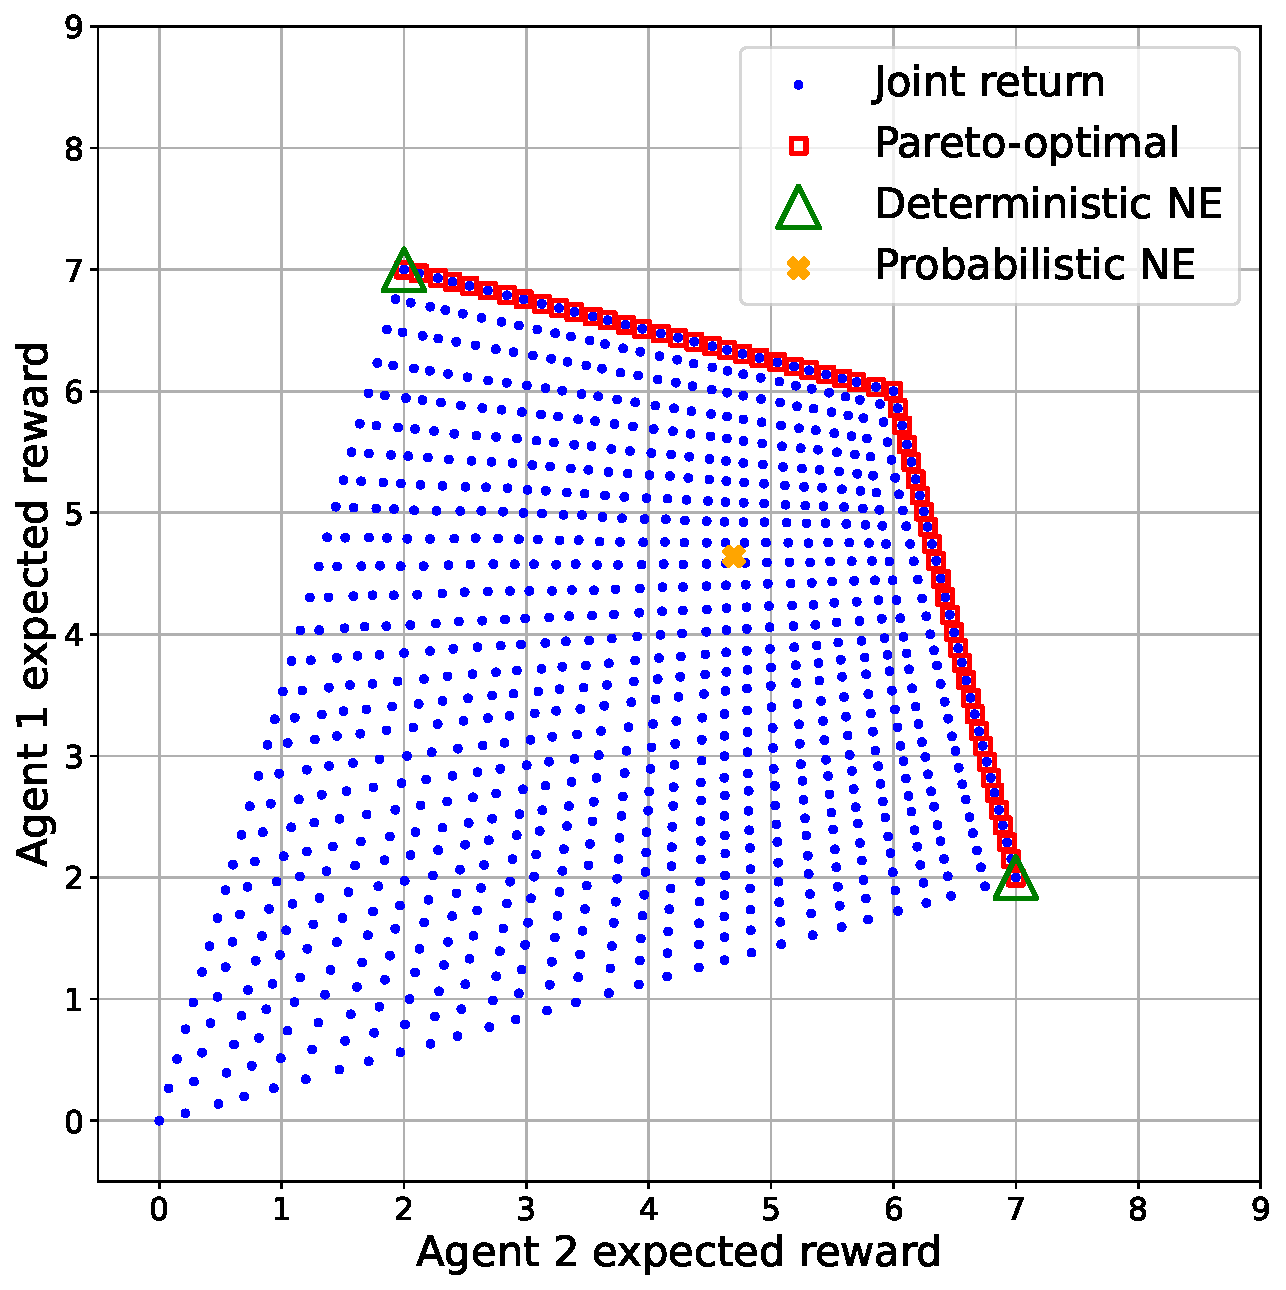
\includegraphics[width=0.8\textwidth, height = 0.8\textheight, keepaspectratio]{images/chapter_4/chicken-po-frontier.pdf}
    \end{figure}
    \end{column}
    \begin{column}{0.5\textwidth}
        \centering
        \vspace{10pt}
        \gamechicken 
        \vspace{10pt}
        \blist
            \item The figure shows the discretized space of joint policies for the chicken matrix game
            \item Each blue dot represents the expected joint return obtained by a joint policy
        \elist
    \end{column}
\end{columns}

\end{frame}

\begin{frame}{Social Welfare and Fairness}

To further constrain the space of desirable solutions, we can consider social welfare and fairness concepts. 

\fat{Welfare optimality:}
\vspace{1pt}
\begin{equation*}
    W(\pi) = \sum_{i \in I}U_i(\pi)
\end{equation*}

\blist
    \item A joint policy \(\pi\) is \fat{welfare-optimal} if \(\pi \in \argmax_{\pi'}W(\pi')\)
\elist

\fat{Fairness optimality:}
\vspace{1pt}
\begin{equation*}
    F(\pi) = \prod_{i \in I} U_i (\pi)
\end{equation*}

\blist
    \item A joint policy $\pi$ is \fat{fairness-optimal} if $\pi \in \argmax_{\pi'}F(\pi')$
\elist

\end{frame}

\begin{frame}{Fairness in Battle of the Sexes}

\begin{columns}
    \begin{column}{0.5\textwidth}
        \begin{figure}
        \centering
        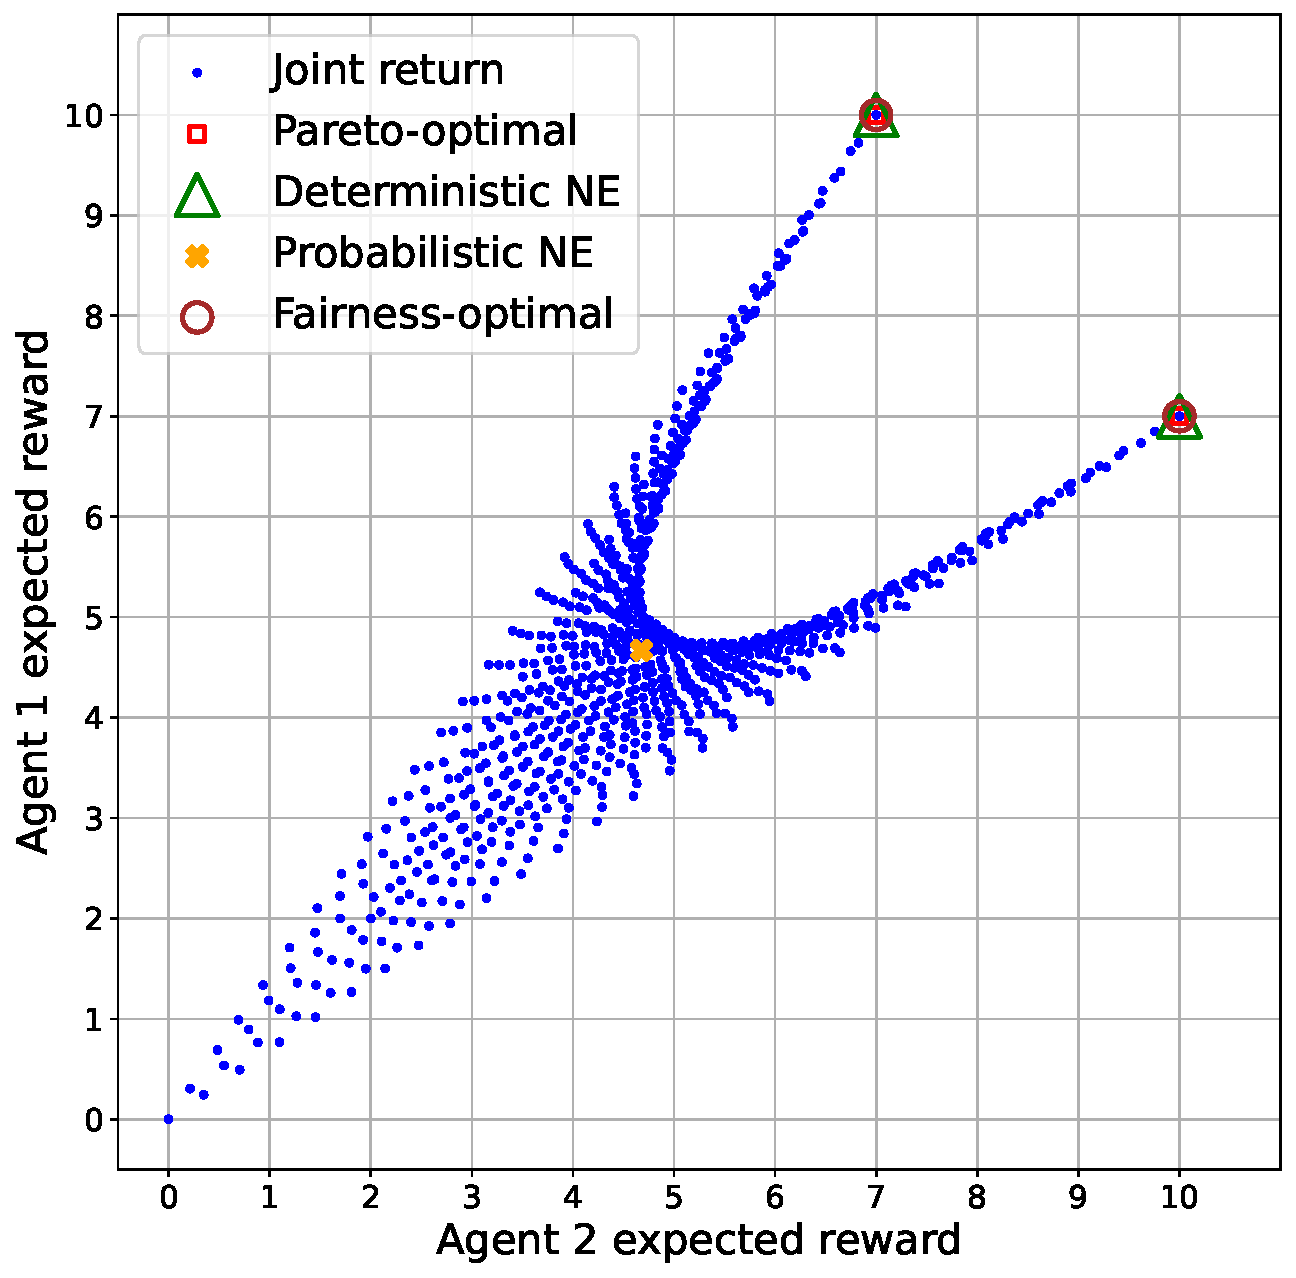
\includegraphics[width=0.8\textwidth, height = 0.8\textheight, keepaspectratio]{images/chapter_4/battlesexes-po-frontier.pdf}
    \end{figure}
    \end{column}
    \begin{column}{0.5\textwidth}
        \centering
        % \fat{Battle of the sexes}
        \vspace{10pt}
        
        \gamebattle
        \vspace{10pt}
        
        \blist
            \item 2 agents agreeing to meet at either location A or B, with each agent having a preference for one or the other location
            \item A, A and B, B are both Nash equilibria and fairness optimal
            \item In the chicken game, there is only 1 Pareto optimal and fairness optimal solution
        \elist
    \end{column}
\end{columns}
    
\end{frame}

\begin{frame}{No Regret}

\fat{Regret} measures the difference between the rewards an agent received versus the rewards it would have received by choosing a different action in past episodes. 
\blist
\item In non-repeated normal-form games (assuming actions of other agents are fixed) \fat{regret} is:
\elist
\begin{equation*}
    Regret_i^{z} = \max_{a_i \in A_i}\sum_{e = 1}^z\left[\mathcal{R}(\langle a_i, a_{-i}^{e}\rangle) - \mathcal{R}_i (a^e) \right]
\end{equation*}

\blist
    \item Let \(a^e\) denote the joint action in episode \(e = 1, ...., z\)
    \item There is no regret if regret is at most 0 as $z \to \infty$ 
    \item  In general-sum games with n agents, the agents have no regret if:
\elist
\vspace{1pt}
 \[
 \forall i: \lim_{z \to \infty} \frac{1}{z}Regret_{i}^{z} \le 0
 \]

\end{frame}

\begin{frame}{No Regret in Prisoners Dilemma}

\begin{figure}[t]
	\centering
	\setstretch{1.1}
	\begin{tabular}{@{} l c c c c c c c c c c @{}}
		\toprule
		Episode $e$ \hspace{5em} 					  & 1 & 2 & 3 & 4 & 5 & 6 & 7 & 8 & 9 & 10 \\
		\midrule
		Action $a^e_1$  			 						 &  C &  C & D  & C  &  D  & D  &  C & D  & D & D \\
		Action $a^e_2$  			 						&  C &  D & C  & D  &  D  & D  &  C & C  & D & C \\
		Reward $\mathcal{R}_1(a^e)$						 & -1 & -5 & 0  & -5 & -3 & -3 & -1 & 0 & -3 & 0 \\
		\midrule
		Reward $\mathcal{R}(\langle C, a^e_2\rangle)$	& -1 & -5 & -1 & -5 & -5 & -5 & -1 & -1 & -5 & -1 \\
		Reward $\mathcal{R}(\langle D, a^e_2\rangle)$	&  0 & -3 & 0 & -3  & -3 & -3 & 0  & 0 & -3 & 0 \\
% RPS
%		Agent 1  & R & P & S & P & S & R & P & S & S & P \\
%		Agent 2  & P & R & R & S & P & R & S & P & R & P \\
%		Reward $\rew_1^t$ & -1 & +1 & -1 & -1 & +1 & 0 & -1 & +1 & -1 & 0 \\
		\bottomrule
	\end{tabular}
 \end{figure}

 \blist
    \item Agent 1 receives total reward \(-21\), always playing D would have resulted \(-15\) 
    \item Thus, \(\text{Regret}_{1}^{10} = -15 + 21 = 6\)
 \elist
    
\end{frame}

\begin{frame}{Generalizing No-Regret to Stochastic Games and POSGs}

For each agent \(i\) we introduce:

\blist
    \item A finite space of policies $\Pi_i$  from which agent $i$ can select a policy
    \item Let $\pi^e$ denote the joint policy from episode $e = 1, ..., z$ with $\pi_i^e \in \Pi_i$ for all $i \in I$
    \item Agent $i$'s regret for not having chosen the best policy across episodes is then defined as
\elist
\[
Regret_i^{z} = \max_{\pi_i \in \Pi_i}\sum_{e = 1}^z\left[U_i(\langle \pi_i, \pi_{-i}^{e}\rangle) - U_i (\pi^e) \right]
\]

\begin{notebox}
    This equation is equivalent to the previous equation for normal-form games if each $\Pi_i$ is a set of \fat{deterministic} policies corresponding to an action $a_i \in A_i$ 
\end{notebox}

\end{frame}

\section{Complexity of Computing Equilibria}

\begin{frame}{Complexity of computing equilibria}
Normal-form games provide a complexity {\it lower bound} for more complex games.
  \begin{itemize}
    \item Two-agent non-repeated zero-sum games have \fat{polynomial-time} minimax solutions via linear programming
    \item Correlated equilibria in non-repeated general-sum normal-form games can also be computed in \fat{polynomial time} via linear programming
    \item Nash equilibria computation is more complex due to the independence assumption  and cannot be done using linear programming
  \end{itemize}
  \begin{problembox}
 	Finding Nash equilibria (NASH problem) is a \fat{total search} problem and has been proven to be\fat{ PPAD complete}
  \end{problembox}
\end{frame}

\begin{frame}{END-OF-LINE PPAD Complexity}

    The END-OF-LINE problem is PPAD complete, meaning all other problems in PPAD, including the NASH problem, can be reduced to it
        % \elist

        END-OF-LINE Definition: Let \( G(k) = (V, E) \) be a directed graph consisting of
        \begin{itemize}
        \item a finite set \( V \) containing \( 2^k \) nodes (each node is represented as a bit-string of length \( k \))
        \item a finite set \( E = \{ (a, b) \mid a, b \in V \} \) of directed edges (from node \( a \) to node \( b \), for \( a, b \in V \)) such that:
        \begin{itemize}
        \item if \( (a, b) \in E \) then \( \exists a' \neq a: (a', b) \in E \) and \( \nexists b' \neq b: (a, b') \in E \)
        \end{itemize}
        \item The goal is to find a node \(e \neq s\) in this graph using two functions:
            \begin{itemize}
                \item Parent(\(v\)) and Child(\(v\)), which return the parent or child node of v, respectively
            \end{itemize}
        \end{itemize}
        
\end{frame}

\begin{frame}{END-OF-LINE - Continued}

\begin{figure}
    \centering
    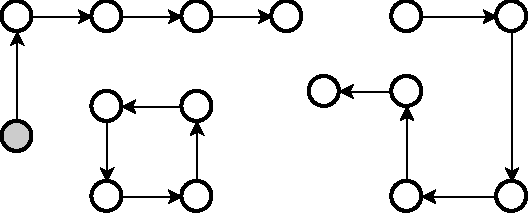
\includegraphics[width=0.4\textwidth, height=0.4\textheight, keepaspectratio]{images/chapter_4/PPAD.pdf}
\end{figure}

\blist
    \item The PPAD "parity argument" ensures the existence of a sink node corresponding to a given source node (in grey)
    \item If a source node is given we know node \(e\) must exist
    \item To find \(e\) we can start at source and repeatedly call Child(v) until we find \(e\)
    \item As the graph scales \(2^k\) this means finding \(e\) may require \fat{exponential time} in the worst case.
\elist
    
\end{frame}

\begin{frame}{Complexity Considerations for MARL}

\blist
    \item<1-> \fat{Reduction to NASH:} Computing Brouwer fixed points and other PPAD problems are reducible to the NASH problem, indicating there are no known efficient (polynomial time) algorithms for solving NASH
    
    \item<2-> \fat{Approximate \(\epsilon\)-Nash Equilibrium:} PPAD-completeness holds for both approximate solutions (\(\epsilon > 0\)) and exact solutions (\(\epsilon = 0\)), with approximations often necessary due to potentially irrational equilibria
    
    \item<3-> \fat{Implications for MARL:} MARL algorithms are unlikely to be a silver bullet for finding Nash equilibria efficiently
    
    \item<4-> \fat{Research Focus in MARL:} Research often targets identifying exploitable structures in certain game types, but MARL may still require \fat{exponential} time when such structures are unavailable.
\elist
    
\end{frame}

\begin{frame}{Summary}

\fat{We covered:}
    \blist
        \item Best Response and minimax
        \item Equilibrium solutions
        \item Additional solution criteria
        \item Complexity of finding Nash equilibria
    \elist

\fat{Next we'll cover:}

    \blist
        \item MARL in games
    \elist
    
\end{frame}

\end{document}

